\documentclass[11pt,twoside,a4paper]{article}

\usepackage{hyperref}
\usepackage{graphicx}
\usepackage{wrapfig}
\usepackage{subcaption}
\usepackage{chngpage}

\begin{document}
%
\includegraphics[width = 40mm]{polito.png}
\title{Machine Learning and Artificial Intelligence Homework 1}
\author{Matteo Borghesi \textit{(s268199)}}
\maketitle

\section{Dataset presentation}
In this report we are going to perform a shallow learning analysis on the Wine dataset. 
%&\footnote{\url{https://scikit-learn.org/stable/modules/generated/sklearn.datasets.load_wine.html#examples-using-sklearn-datasets-load-wine}}
This dataset contains results of a chemical analysis of wines grown in the same region in Italy by three different cultivators. Although it features thirteen different measurements regarding different constituents, we will consider only two of them, which are the Alcohol and the Malic Acid. Our goal is to be able to predict which cultivator produced a certain wine just by looking at these two attributes. Such a task is called classification, which is a type of supervised learning problem, since the training samples are already 'labeled' with the right outcome.

In order to do that, we will randomly split the data in a training set, a validation set and a test set, with proportion 5:2:3. Since the dataset contains 178 samples overall, there will be 89 samples in the training set, 35 in the validation and 54 in the test set.
In section~\ref{CV} we will then merge the training and the validation set and proceed with cross validation on the resulting set.\newline
In order to prevent one attribute from overpowering the other one in the analysis, the samples are normalized according to the mean and the variance as computed on the training and validation set.

\section{K-nearest Neighbors}
\label{KNN}
As a first step, we apply the K-nearest Neighbors (a.k.a. KNN) algorithm to the Wine dataset. The idea behind said algorithm is to assign the class labels to the test items basing on their 'proximity' to the training samples. In particular, the label that occurs most often in the \emph{k} 'nearest' samples is chosen as prediction. The proximity between two samples can be measured according to different metrics: in our analysis - as it is mostly the case - we use the Euclidean distance, i.e. the norm of the difference between the two sample vectors.

We apply our analysis four times for different values of the parameter \emph{k} (respectively 1, 3, 5 and 7). The result of the training phase is shown in fig.~\ref{fig:knnPred}, with the dots representing the training items. The background colors on the other hand signal which class is assigned to test samples whose attributes fall within that area. As it can be seen on the plots, as \emph{k} increases the boundary lines become more uniform, since they depend less on single or few samples lying in an area where the majority of the items belong to a different class. Although this reduces the risk of overfitting the data provided, it may also reduce the model's capability of recognizing particular structures in the data.\newline
Indeed, if we measure the accuracy of the model to varying of \emph{k} (see fig.~\ref{fig:knnScore}) we notice that it's not necessarily the highest \emph{k} that makes the best prediction. This balance between overfitting and underfitting the data, known as bias-variance tradeoff, is inherent to most statistical learning methods.

\begin{figure}[!b]
  \begin{center}
  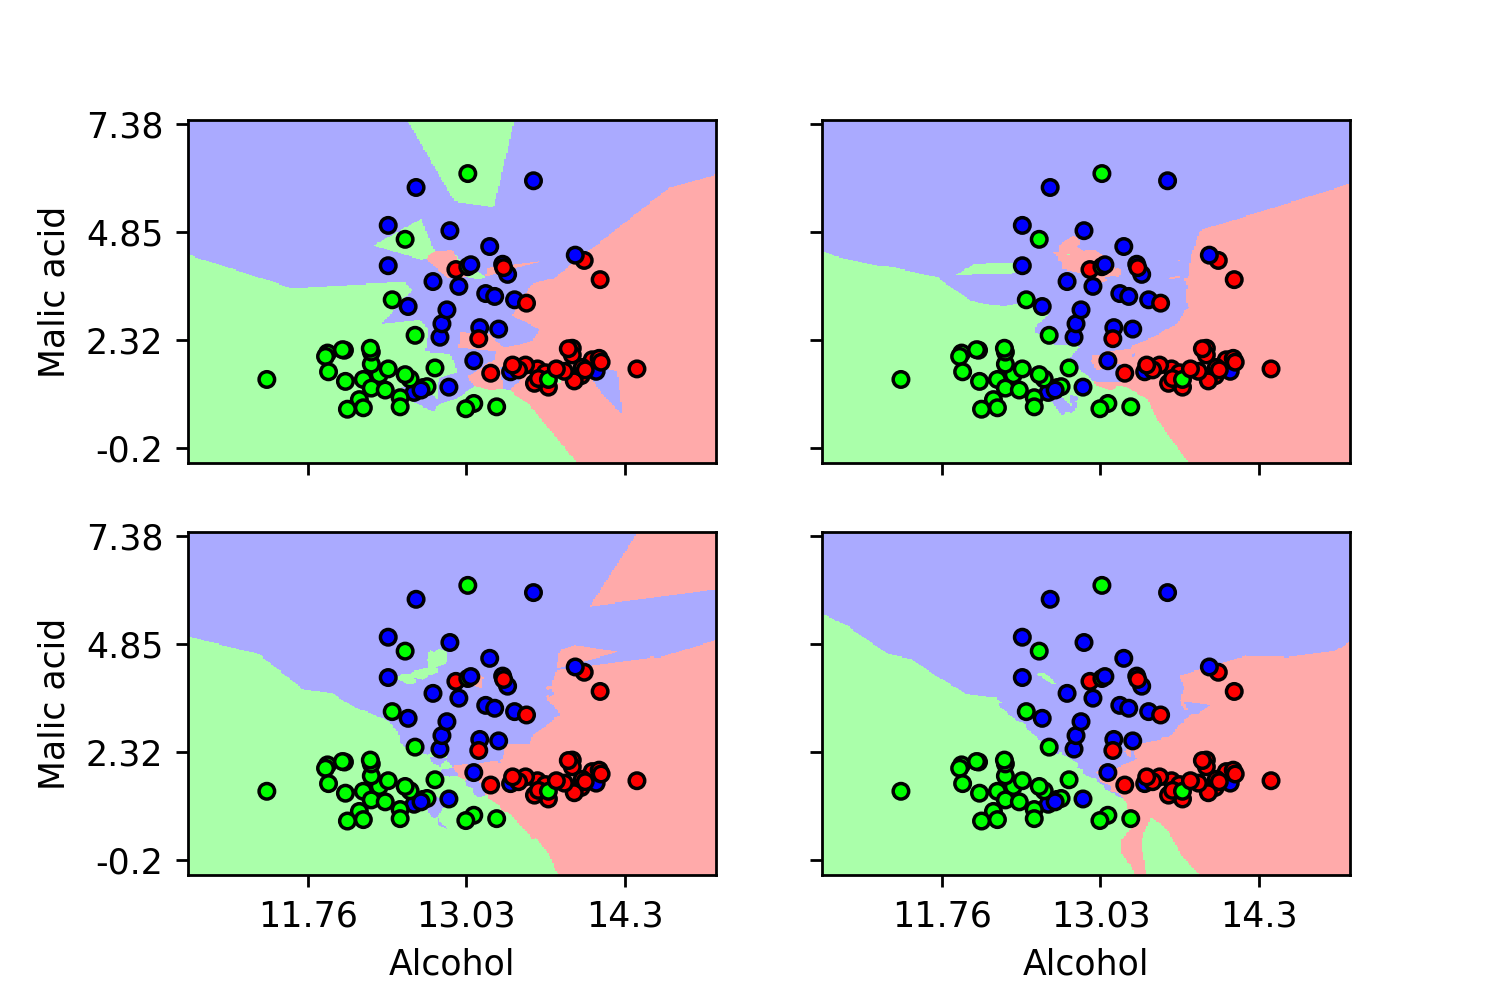
\includegraphics[width=0.8\linewidth]{knnPredPlot.png}
  \caption{Knn analysis}
  \label{fig:knnPred}
  \end{center}
\end{figure}

As intuition suggests, we choose as optimal the value of \emph{k} that maximizes the accuracy of the model on the validation test, in this case \emph{k}=7. Once we have done that, we can estimate the reliability of the model by measuring its accuracy on the test set, whose data have been kept out all through the process of model selection. Clearly, the accuracy measured both on the validation and on the test set depends on the split performed during the first stage, which we said to be random: the smaller are the sets, the higher is the variance of these measures. In our case, the test set contains 89 items, and therefore the accuracy measures are prone to instability.\newline
After evaluating the chosen model on the evaluation test, the resulting accuracy is 0.74.


\section{Linear Support Vector Machines}
\label{SVM}
In the second stage of our classification analysis, we use a method called Support Vector Machines (SVM), which aims to find linear decision boundaries in the plane of the feature vectors, so that all points belonging to the same class lie on the same side of the boundary. Furthermore, SVM is designed to maximize the minimum distance between the linear separator and the points of all classes.\newline
If the problem is not linearly separable, it is possible to introduce a parameter \emph{C} in the model, called 'slack variable', which is a degree of tolerance for points that lie beyond the decision boundary, and so belong to a different area than the one of their class.

\begin{figure}[!b]
  \begin{center}
  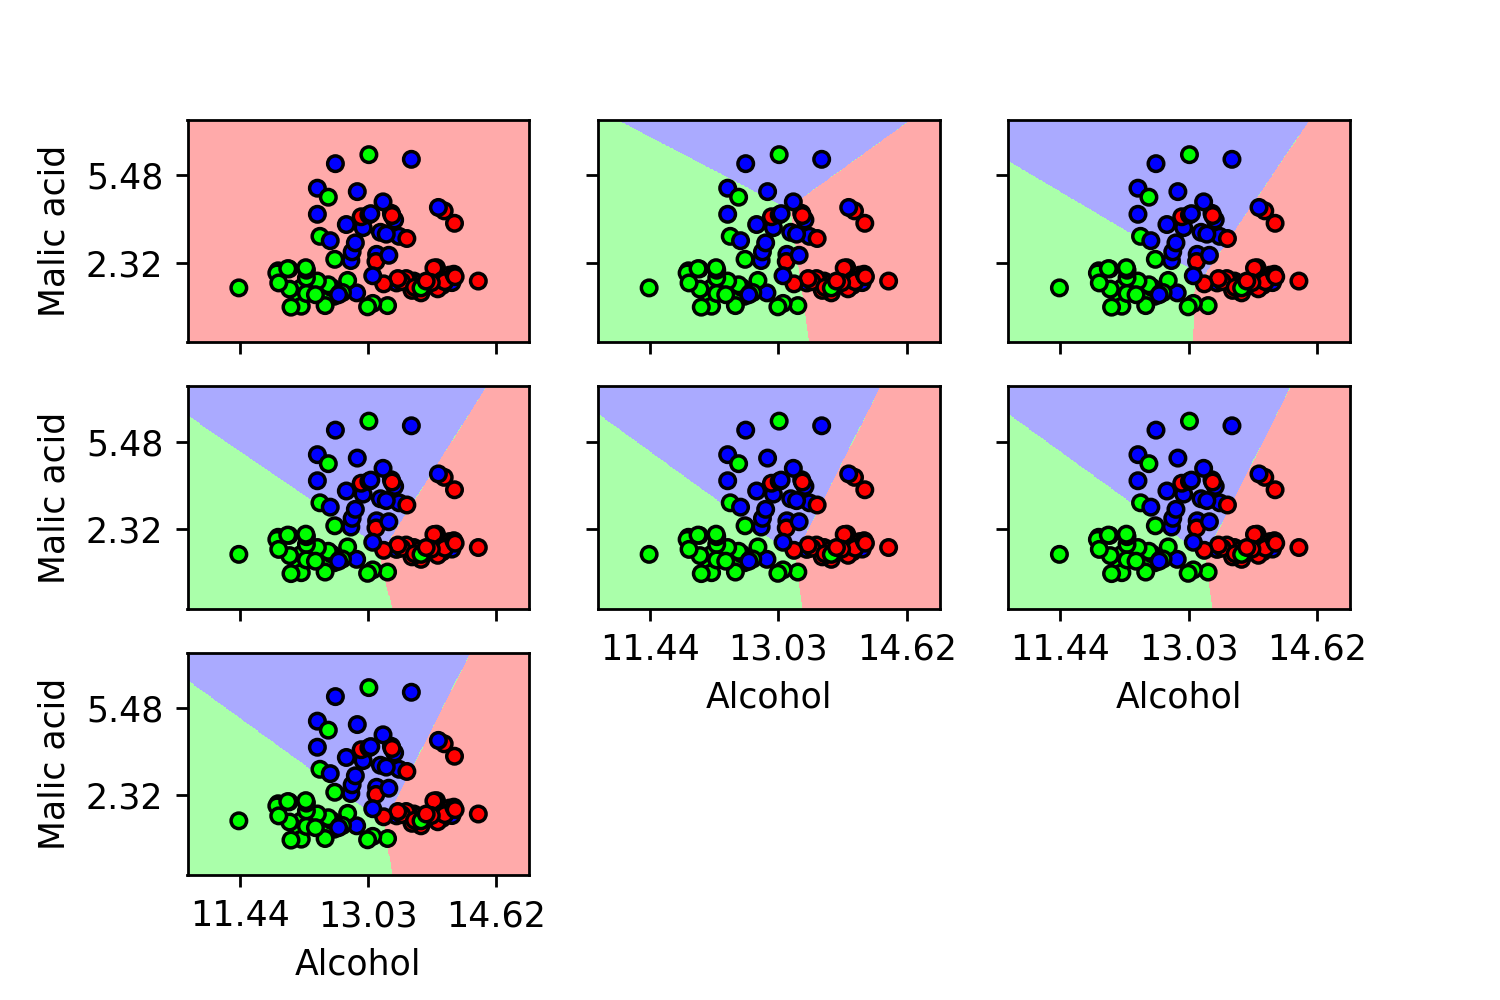
\includegraphics[width=\linewidth]{linearPredPlot.png}
  \caption{Linear SVM analysis}
  \label{fig:linearPred}
  \end{center}
\end{figure}

\begin{figure}[]
    \centering
    \begin{subfigure}{0.7\textwidth}
	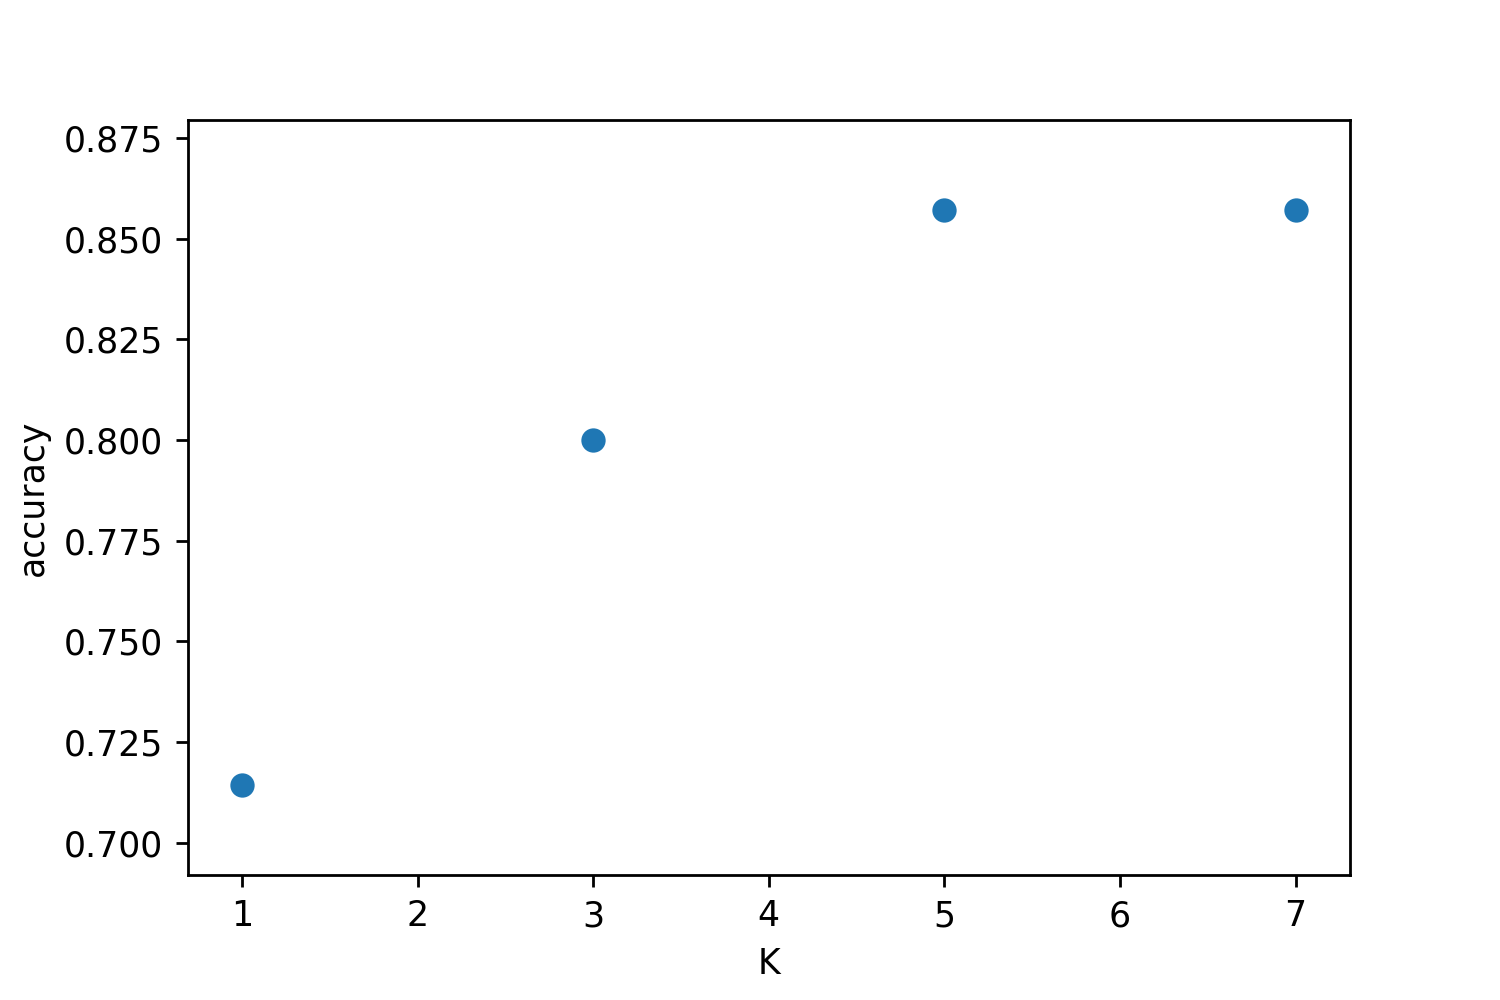
\includegraphics[width=\linewidth]{knnScorePlot.png}
        \caption{}
        \label{fig:knnScore}
    \end{subfigure}
    \begin{subfigure}{0.7\textwidth}
	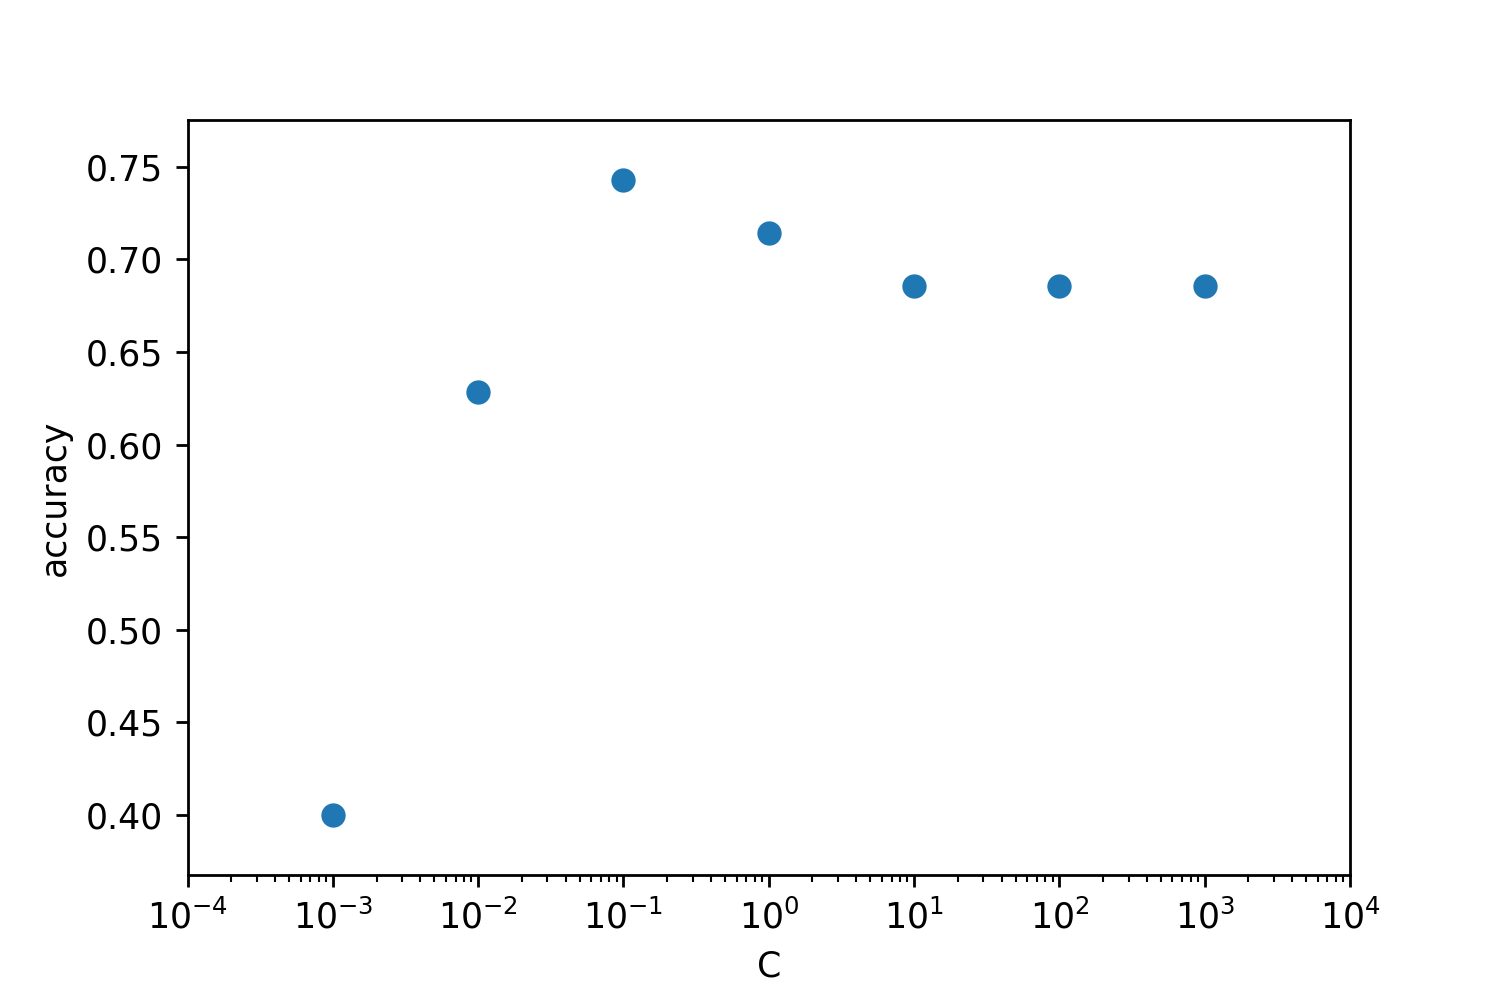
\includegraphics[width=\linewidth]{linearScorePlot.png}
        \caption{}
        \label{fig:linearScore}
    \end{subfigure}
    \begin{subfigure}{0.7\textwidth}
        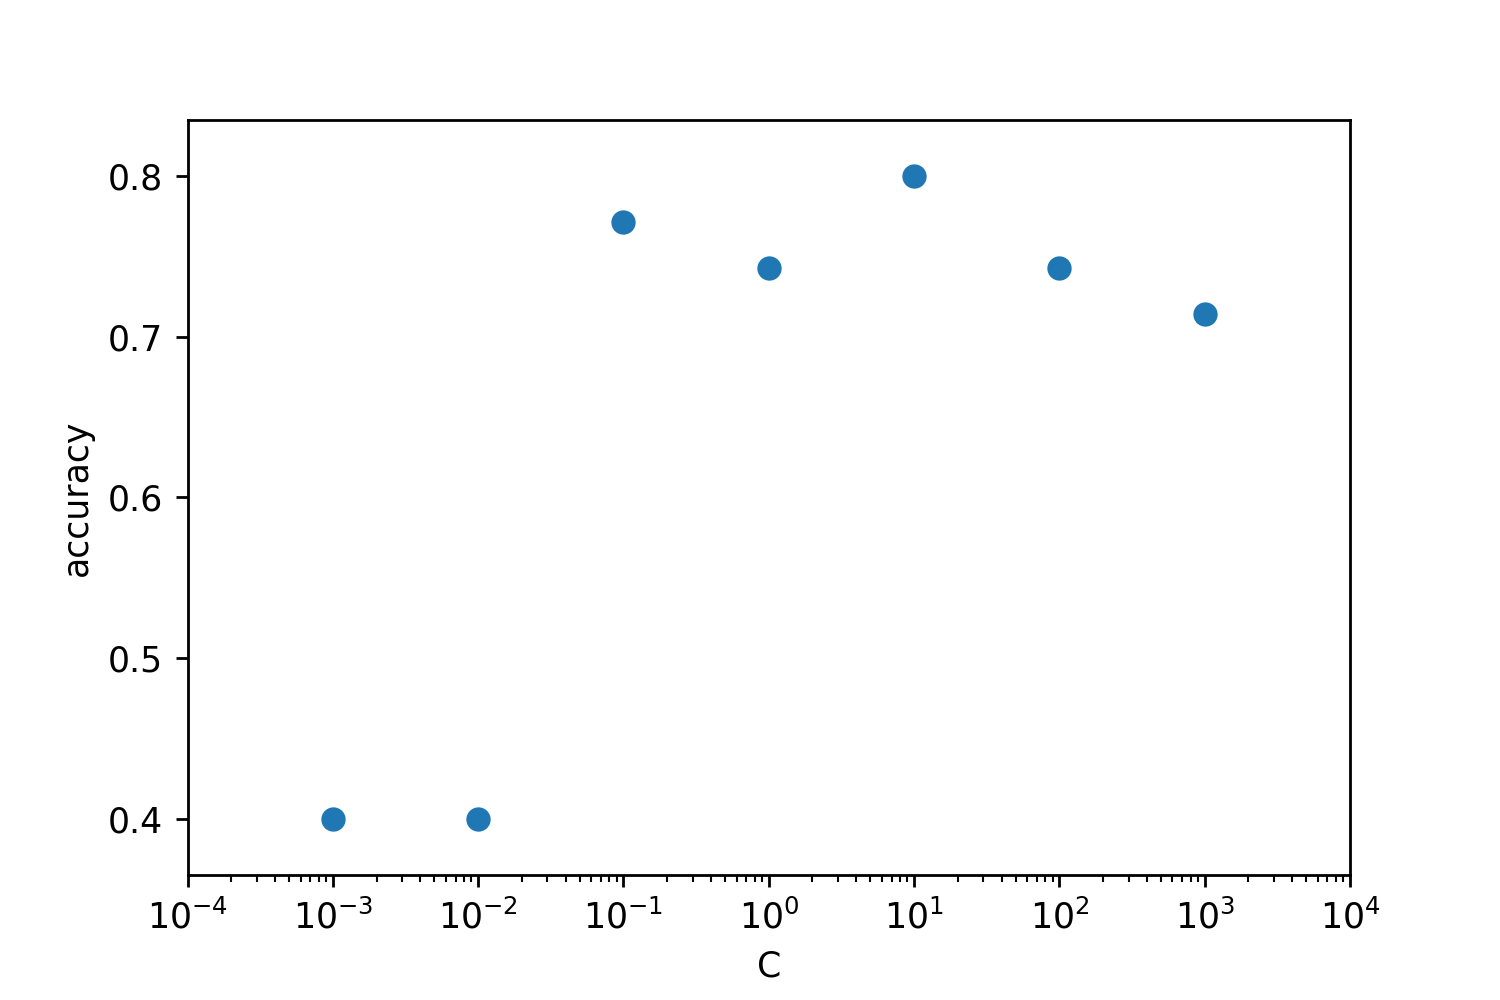
\includegraphics[width=\linewidth]{rbfScorePlot.png}
        \caption{}
        \label{fig:rbfScore}
    \end{subfigure}%
    \caption{Accuracy on the validation set in KNN (a), linear SVM (b) and rbf SVM (c)}
\end{figure}

As we already did for KNN, we build classifiers for multiple values of \emph{C} (here 0.001, 0.01, 0.1, 1, 10, 100, 1000) basing on the training set and evaluate them on the validation set, then we choose the one with the best score and assess its reliability by means of the test set.\newline
The resulting decision boundaries are plotted in fig.~\ref{fig:linearPred}. For the smallest value of \emph{C}, the problem is not linearly separable into three classes, because the model admits by construction only a low level of flexibility in accepting wrong labelings. When \emph{C} gets higher, it is possibile to find linear separators that satisfy the condition for all the points. However, beyond a certain threshold the model remains unchanged, since higher values of the slack variable do not bring any extra benefit to the model. 

The same can be noticed in fig.~\ref{fig:linearScore}, which plots the accuracy on the validation set for the different values of \emph{C}. As the model becomes able to linearly separe the data, the accuracy has a boost, whereas after that it reaches a knee, beyond that it remains stable or even falls, as in this case. We finally pick the model that performs best on the validation set and estimate its accuracy on the test set, which turns out to be 0.777.

\begin{figure}[!b]
  \begin{center}
  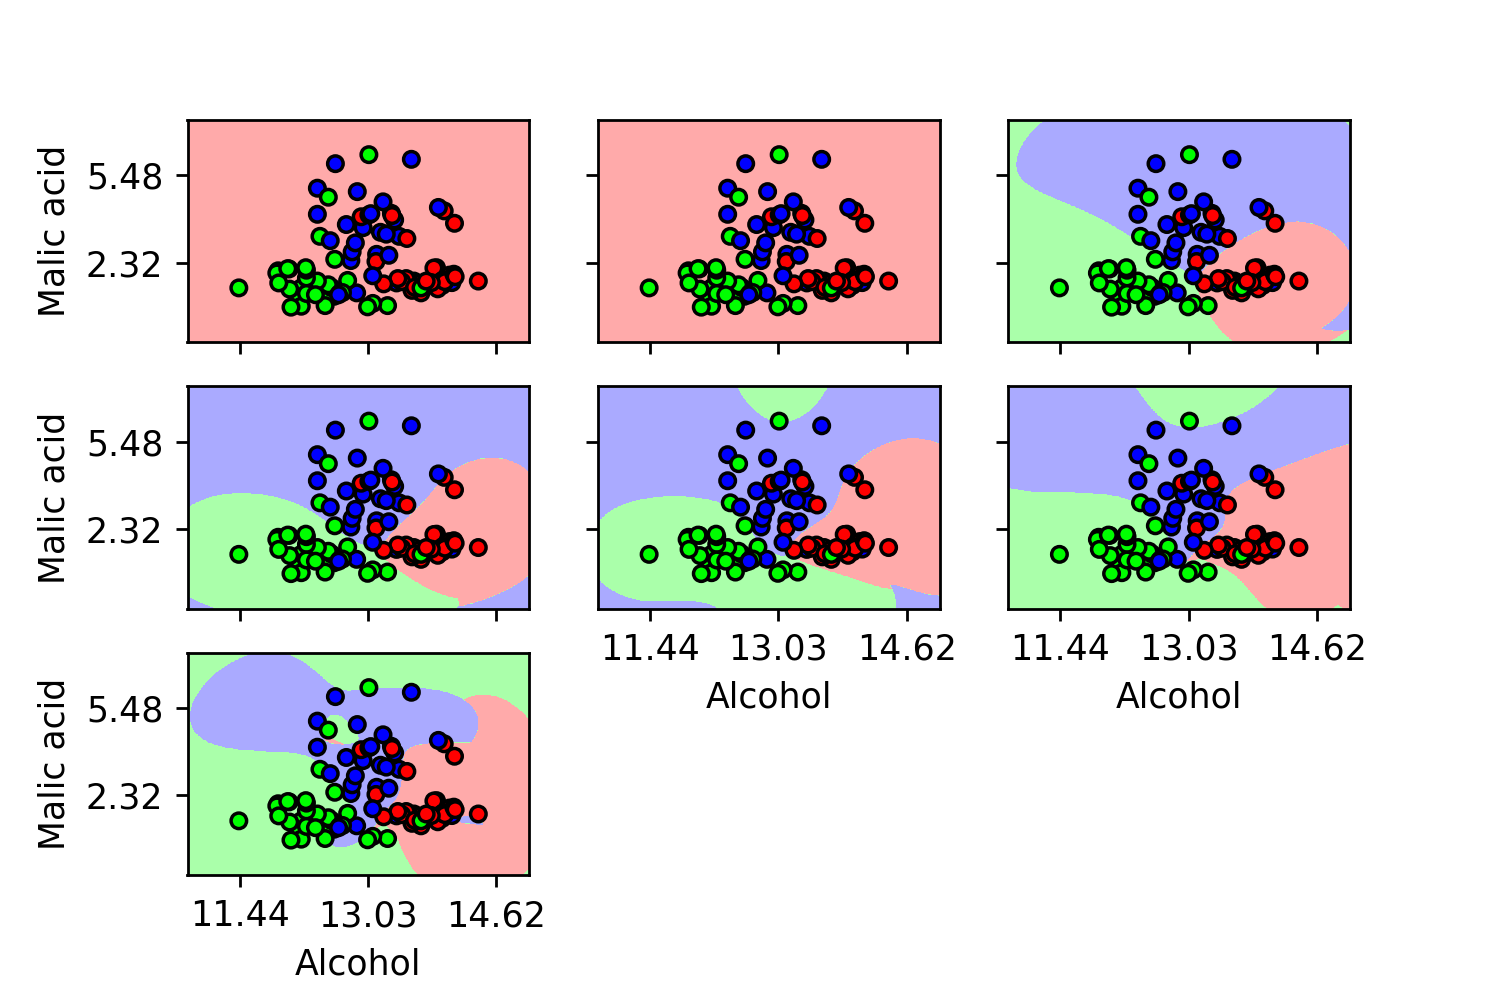
\includegraphics[width=\linewidth]{rbfPredPlot.png}
  \caption{Kernel SVM analysis}
  \label{fig:rbfPred}
  \end{center}
\end{figure}

\section{Kernel Support Vector Machines}
\label{RBF}
Sometimes having to linearly separe the dataset in the feature plane can get quite complicated. In this cases, plotting the data into some higher dimension can help overcoming such problem. For example, if we could project our two-dimensional data into a 3D space it would be possible to use a plane to separe them, instead of a line: this technique is called the \emph{kernel trick}. There are different functions commonly used to kernelize a problem: in our analysis we are going to use the Radial Basis Function, also called RBF.

As in sec.~\ref{SVM}, it is possible to introduce a slack variable \emph{C} to account for samples lying by a certain amount beyond the decision boundary of their class. Again, we repeat our training for \emph{C} equal to 0.001, 0.01, 0.1, 1, 10, 100 and 1000. As any other kernel function, RBF enlarges the space by constructing new features out of the existing ones; however, since those functions are mainly not linear, when we look at the decision boundaries plotted onto the original hyperplane they don't appear as linear anymore, either. The decision boundaries resulting from our models together with the training data are plotted in fig.\ref{fig:rbfPred}.\newline
Also here it's important to find a balance point to optimize the bias-variance tradeoff: as fig.~\ref{fig:rbfScore} shows, in this case the best value for \emph{C} coming out from validation is 10. When we evaluate the according model on the test set, it performs with an accuracy of 0.777, just as much as in the linear case.


\section{Grid Search}
We have seen that machine learning models are controlled by user-defined parameters. In the example of KNN in sec.~\ref{KNN} it was the number \emph{K} of neighbors that were taken into account to make the prediction, while in the case of SVM in sec.~\ref{SVM} and \ref{RBF} we have played with the slack variable \emph{C}.\newline
In order to make a more reliable prediction, it is advisable to perform the training over many or even all of the parameters that may influence the behavior of the model. It is possible then to assess through validation which tuple of parameters has the most satisfactory score, so that it can be included in the final model to be delivered. Such an analysis is called Grid Search, since all possible conbinations are layed out in a grid, or more simply in a matrix, which displays their performance at validation.

\begin{figure}[!b]
    \begin{center}
    \begin{subfigure}{0.48\textwidth}
	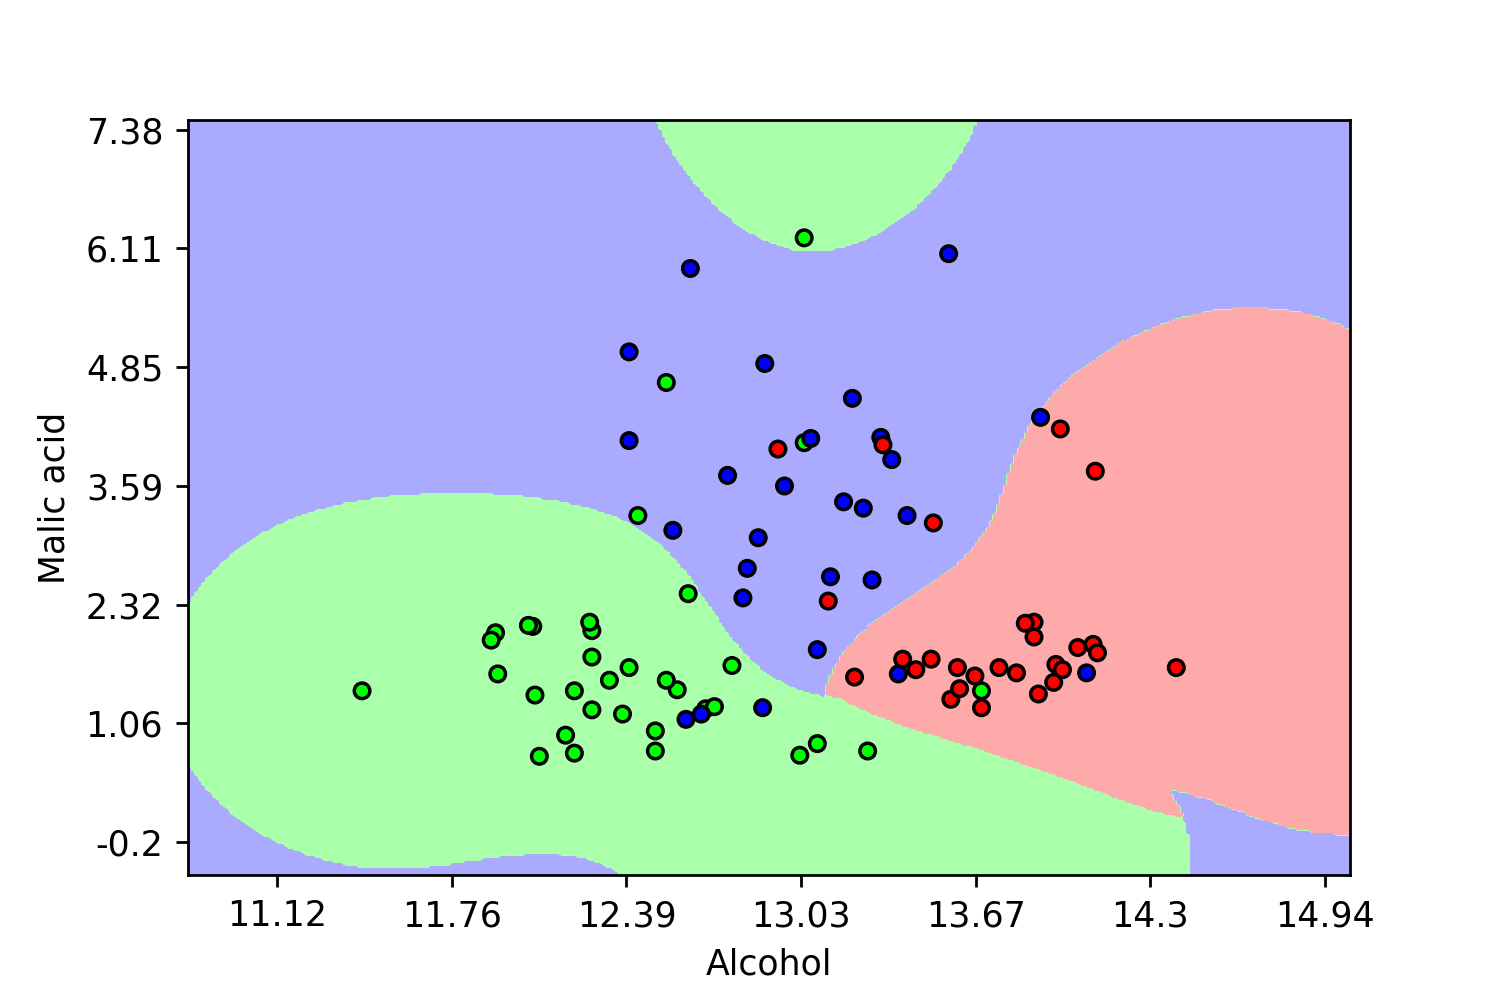
\includegraphics[width=\linewidth]{gridPredPlot.png}
        \caption{}
        \label{fig:gridPred}
    \end{subfigure}
    \hspace{\fill}
    \begin{subfigure}{0.48\textwidth}
	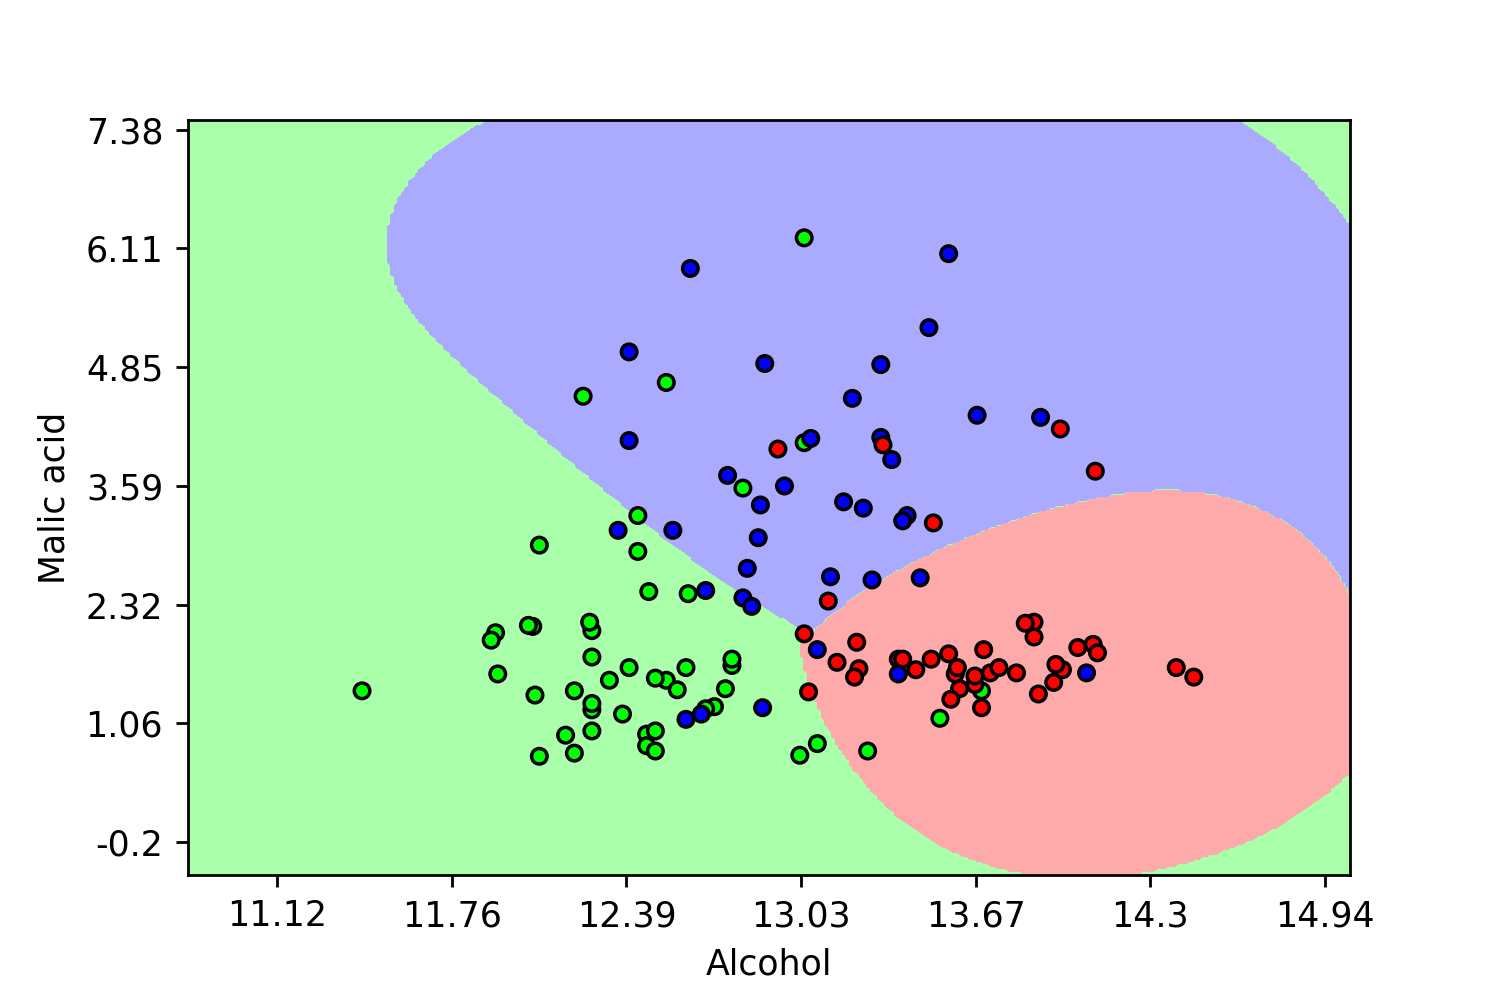
\includegraphics[width=\linewidth]{cvGridPredPlot.png}
        \caption{}
        \label{fig:cvGridPred}
    \end{subfigure}
    \caption{Decision boundaries in the models resulting from grid search (a) and grid search with 5-fold CV (b)}
    \end{center}
\end{figure}

In the context of the Wine dataset, grid search can be carried out on the support vector classifiers, which indeed have more parameters than just \emph{C}. In this section we are going to repeat the training phase in the case of the RBF kernel for all values of \emph{gamma}, which are 'auto' and 'scale'. The purpose of this parameter is to control how much the new feature computed by the RBF funcion is going to influence the decision boundary. Clearly, the analysis in sec.~\ref{RBF} must have had some value for \emph{gamma} already, which was by default 'auto': hence we only have to carry out the training for \emph{gamma}='scale'.

After having computed the accuracy of all combinations, we choose the model with the highest score and assess it on the test set, in order to provide a reliable estimation of our result. In this case the final model will use \emph{C}=0.1 and \emph{gamma}=scale, and has a test accuracy of 0.777. This is no wonder, since it turns out to be the same model chosen in sec.~\ref{RBF}, as it can be seen also by looking at the decision boundaries (fig.~\ref{fig:gridPred}). The reason for that is that apparently there was no value of \emph{C} with \emph{gamma}=scale which performed better, so the algorithm sticked with the same values also after the more extended grid search.


\section{Cross validation}
\label{CV}
So far we have made a strict separation between the training and the validation set. However this is somehow an 'artificial' division, which we can look at just as a choice in the methodology followed to carry out the analysis. On the contrary, the division between the test set and the other data (training and validation set) is a must-have in order to preserve the scientificity of the work.

In this section we are going to look at another method to deal with train and validation data, called Cross Validation (CV). Such method doesn't perform a once-and-for-all split between training and validation data; instead the data are split into \emph{K} buckets of equal size. The training process is then repeated \emph{K} times, each time using one bucket as validation set and the rest of the data as training set. At the end, the iteration that features the highest accuracy is chosen and its reliability is estimated on the test set as usual.

We can now combine this concept with the grid search from last section: we perform a model selection using grid search, but each combination is evaluated through 5-fold CV (i.e. \emph{K}=5), instead of just estimating its accuracy on a statically defined validation set. The resulting decision boundaries are plotted in fig.~\ref{fig:cvGridPred}, and its test accuracy amounts to as much as 0.814. This is higher than the result obtained in the last section, which used the same training method but a different validation strategy, because repeating the training phase different times, each time with different training and validation sets, allows to better tune the output vector to the data, so that it is able to better predict new samples.


\section{Principal Component Analysis}
In this last section, we explore a different approach to the analysis of the data contained in the Wine dataset. In fact, at the beginning we have decided to take into consideration only two attributes for the sake of our work, specifically Alcohol and Malic Acid. Yet it could be that other attributes are more significant in the pursuit of our goal, that is the prediction of which cultivator has produced a certain wine. Even more, the feature vectors could be represented using a different base than the standard one, and we could find a base such that its first two coefficients lead to a better prediction than sofar.\newline
This concept is at the base of the Principal Component Analysis (PCA) algorithms, which select a new base to represent the samples in which the first basis vectors retain the most variance, i.e. the most information. The major drawback of this strategy is that the basis vectors are not bounded anymore to a human-relevant attribut (e.g. Alcohol or Malic Acid), but instead they represent a linear combination of various features, which makes the models (and as a consequence the plots) more difficult to interpret.

We therefore select the first two components in the basis computed through PCA and represent our original 89 train samples in the new basis. After that we build prediction models using KNN, linear SVM and RBF-kernelized SVM. For an easier comparison, we use in each model the parameters chosen at validation in sec.~\ref{KNN}-\ref{RBF}, which were also used to perform the test. For this reason, and for the fact that the training set has the same size as before, it makes sense to compare the test scores of the resulting models with the ones obtained in the previous sections.\newline
The outcomes are shown in tab.~\ref{tab:accuracy}. Generally speaking, PCA brings to an improvement with regards to KNN and kernel SVM, while the accuracy remains stable in the case of linear SVM. However, the highest score among all techniques presented in this report is reached by the grid search with cross-validation from sec.~\ref{CV}: of course, it would still be possible to combines this method with PCA and to look if its prediction rate can be still improved.


\begin{table}[!h]
  \begin{adjustwidth}{-.5in}{-.5in}
  \begin{center}
    \begin{tabular}{l | c | c | c | c}
       & normal & grid search & grid search with CV & PCA  \\
      \hline
      KNN & 0.740 & - & - & 0.796 \\
      linear SVM & 0.777 & - & - & 0.777 \\
      kernel SVM & 0.777 & 0.777 & 0.814 & 0.796 \\
    \end{tabular}
    \caption{Comparison of test accuracies}
    \label{tab:accuracy}
  \end{center}
  \end{adjustwidth}
\end{table}

\end{document}

